\documentclass{scrbook}
\usepackage[utf8]{inputenc}
\usepackage{graphicx}

\title{SpaceWalk The Game}
\author{Péter Bence, Vasánszky Milán, Székely katalin, Tóth Balázs}
\date{October 2022}

\begin{document}

\maketitle

\section{Alapinformációk} 
Ez a specifikáció egy szöveges, szerepjátékos űrkalandjátékhoz készült. A játék- ban mozoghatsz szobáról szobára, gyűjthetsz tárgyakat és új utakat nyithatsz meg a játék világának felfedezéséhez. Találkozhatsz és interakcióba léphetsz NPC-kkel. A program a felhasználótól vár egyszerűbb parancsokat, amelyeket később eseményként megjelenít. A történet X mélységű. Az alkalmazás a felhasználó által adott helytelen bemenetre hibaüzenettel válaszol.

\section{Történetvázlat}
Az év 2094. A mesterséges intelligencia teljes mértékben átvette az irányítást a Föld nevezetű bolygó felett 30 évvel ezelőtt. De nem úgy ahogy gondolod kedves PLAYERNAME. 2064-ben kifejlesztették az Oázis AI-t, ami egyedül azt a cél szolgálja, hogy az emberek kényelemben éljenek. A tökéletes utópisztikus világ, ahol az emberek azért jönnek a Földre, hogy jól érezzék magukat, azzal foglalkozzanak, amivel csak akarnak, és akkor, amikor akarnak. Minden unalmas és monoton feladat elvégzését átvették a robotok és az OAI. Ebbe beletartozik a teljesen automatikus házvezetés, takarítás, bevásárlás, és még a főzés is. Nem kevés következménnyel járt ez az átállás. Beolvasztották az összes fegyvert, megszüntették az autókat, és csak is mindenki buszokkal, vagy kijelölt szállítási eszközzel közlekedhet. A 2045-ös jégkorszak után nagymértékben megcsappant a Föld lakossága. A tervezett 9,44 milliárd ember helyett kevesebb, mint 1 milliárd maradt.

\section{Használati esetek}
\begin{table}[h] \centering
    \caption{Használati esetek}\label{tab:usecasetable}
    \begin{tabular}{@{}ll@{}}
        \emph{Eset} & \emph{Leiras}\\ \hline
        Move         & Mozgas szobarol szobara\\
        Search room  & Kutasd at a szobat, itemek es NPC-k utan\\
        Pick up item & Vegyed fel a talalt targyat\\
        Interact with NPC & Beszelj a talalt NPC-vel\\
        Accept mission & Fogadd el az NPC kuldeteset
    \end{tabular}
\end{table}

\graphicspath{{../Planning/}}
\begin{figure}\centering
    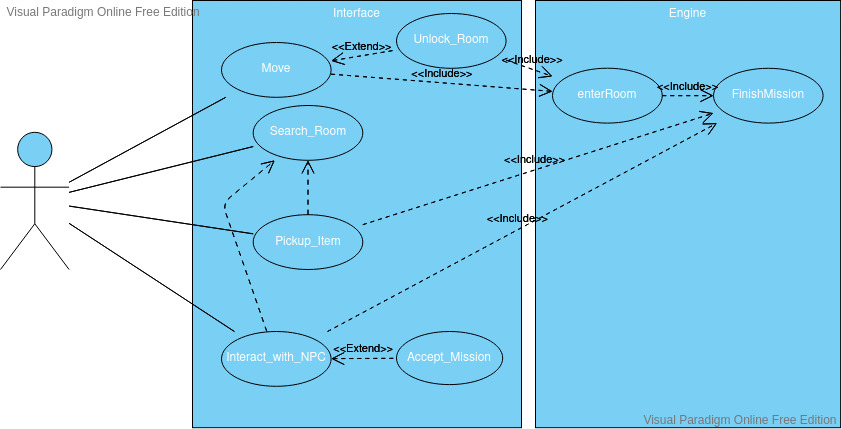
\includegraphics[width=1.0\columnwidth]{Functional_UseCase.jpg}
    \caption{Functional Use Cases}\label{fig:1}
\end{figure}

\begin{figure}
    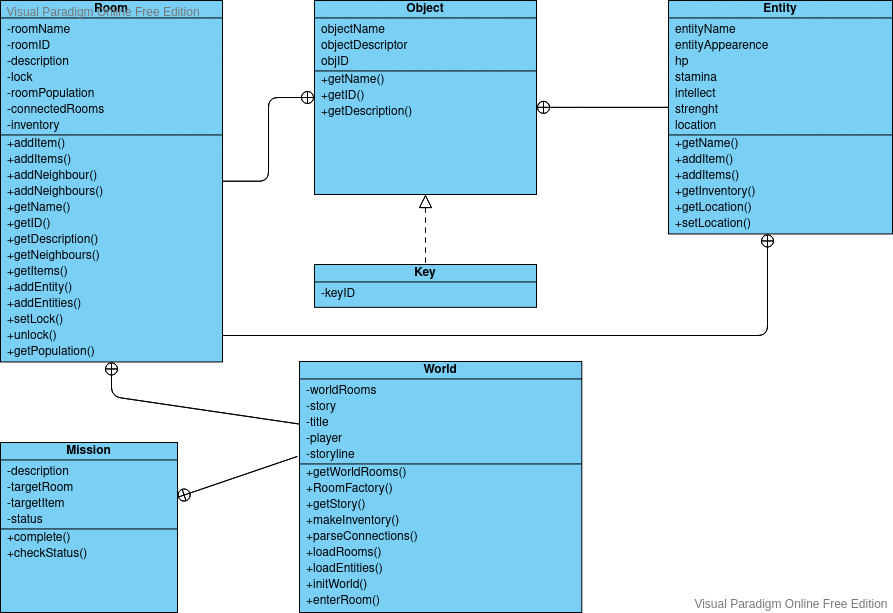
\includegraphics[width=1.0\columnwidth]{Class_Architecture.jpg}
    \caption{Class Architecture}\label{fig:2}
\end{figure}

\begin{figure}
    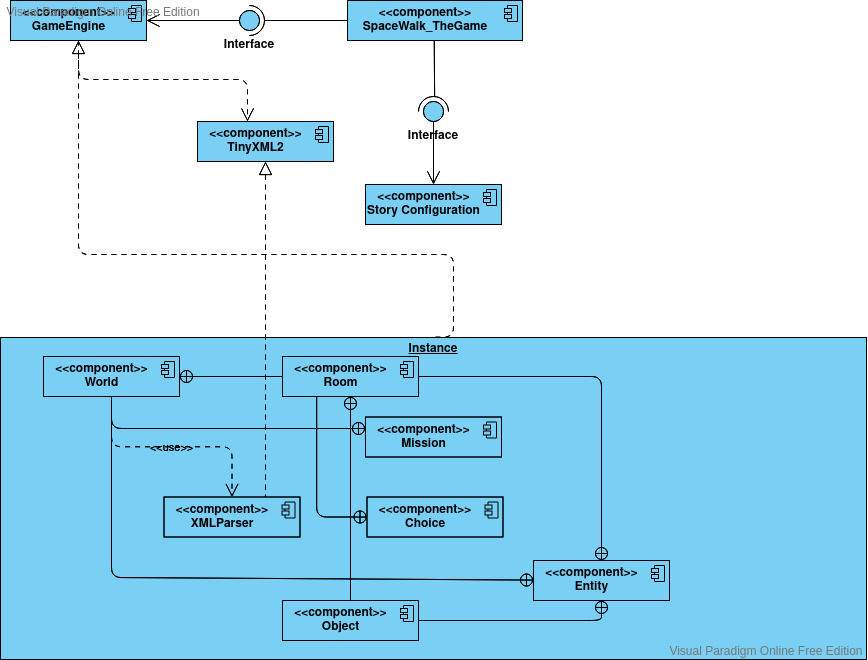
\includegraphics[width=1.0\columnwidth]{Component_Connection.jpg}
    \caption{Component connection}\label{fig:3}
\end{figure}

\begin{figure}
    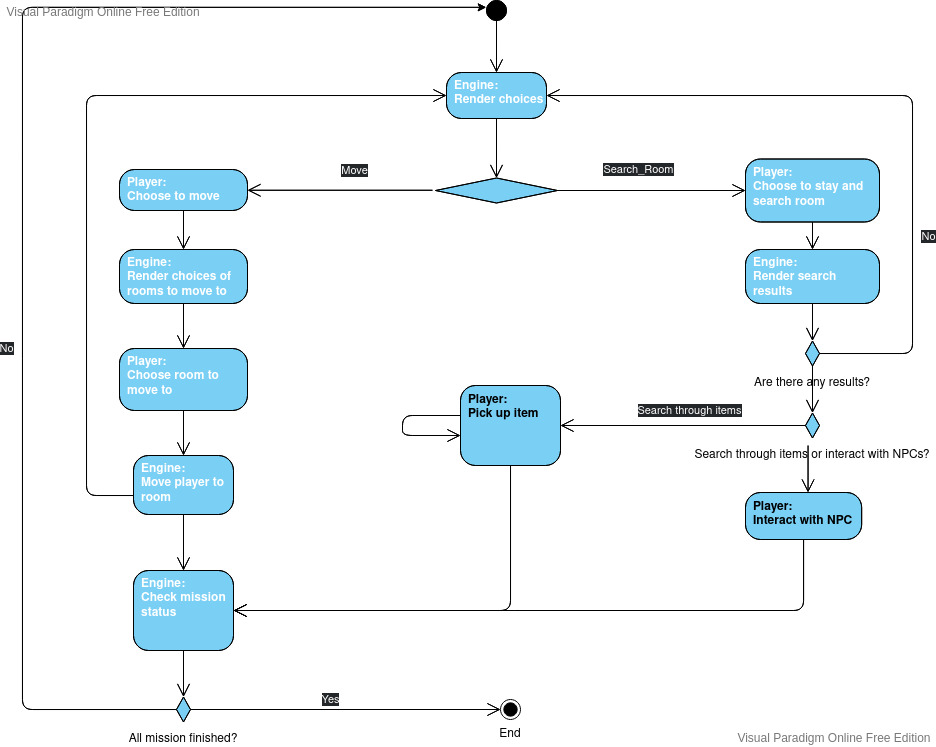
\includegraphics[width=1.0\columnwidth]{GameLoop_ActivityDiagram.jpg}
    \caption{Gameloop Activity Diagram}\label{fig:4}
\end{figure}

\end{document}